\documentclass[a4paper,12pt]{article} %style de document
\usepackage[utf8]{inputenc} %encodage des caractères
\usepackage[french]{babel} %paquet de langue français
\usepackage[T1]{fontenc} %encodage de la police
\usepackage[top=2cm,bottom=2cm,left=2cm,right=2cm]{geometry} %marges
\usepackage{graphicx} %'affichage des images
\usepackage{algorithm2e}
\usepackage{listings}

\usepackage{enumitem}
\usepackage{verbatim}

\usepackage{hyperref}
\hypersetup{colorlinks = True,
	linkcolor=blue}

\usepackage{amssymb} %'Les ronds et carrés avant les listes
\usepackage{lastpage}
\usepackage{fancyhdr}
\pagestyle{fancy}

\renewcommand{\footrulewidth}{0.2pt}
\renewcommand{\headrulewidth}{0pt}
\fancyfoot[L]{Rapport Groupe 2,2021-2022 }
\fancyfoot[R]{page \thepage} 
\fancyfoot[C]{} 


\title{Simmulation du jeu de la vie - conception logiciel  2022-2023 }
\author{mis en page par \\
   DIARE Youssouf  22008756\\
   OLANGASSICKA Franck  22112035\\
   KONE saybou 21911516\\
   YATTOURA Mohamed 22012262\\
   L2 info,\\
   Groupe 2 \\}
 

\begin{document} %début du document

\begin{titlepage}
\maketitle

\includegraphics[scale=1]{images/LogoUNICAEN.png}
\centering

\end{titlepage}

\renewcommand*
\contentsname{Sommaire}
\tableofcontents

\clearpage
\section{Introduction  }
L’unité d’enseignement Projet 1 a pour objectif de nous faire comprendre le concept de la programmation orientée objet, nous initier aux implémentations des algorithmes  et parfaire notre maitrise de java. \\

Pour cela des groupes de 4 d’étudiants ont été formés et plusieurs projets ont été proposés, Éditeur de livres dont vous êtes le héros, Interpréteur de systèmes de Lindenmeyer, Interpréteur de programmes chimiques, etc.
		Notre groupe a choisi le projet Jeu de la vie. 
\subsection{Présentation du projet}
Le jeu de la vie est un projet informatique qui simule l’évolution des cellules d'une grille bidimensionnelle .Il a été crée par le mathématicien Jhon Horton Conway en 1970. Ce jeu ce déroule en plusieurs étapes ou générations , au départ l'utilisateur définit une grille de cellules qui peuvent être vivantes ou mortes et à chaque étape les cellules évoluent en fonction des règles suivantes :
\begin{itemize}
\item Une cellule vivante qui a moins de deux cellules voisines meurt, par solitude.
\item Une cellule vivante qui a plus de trois cellules voisines vivantes meurt, par surpopulation.
\item Une cellule morte qui a exactement trois cellules voisines vivantes devient une cellule vivante, par reproduction.
\item Les cellules vivantes qui ont deux ou trois cellules voisines vivantes restent en vie.
\end{itemize}
\subsection{Objectif du projet}

Le but de ce projet est de développer un programme permettant  la simulation de
l’évolution de cellule sur une surface.  Dans un premier temps, il s'agit de développer le moteur du jeu (cf. règles) puis le doter d'une interface graphique permettant la visualisation des générations. Dans un second temps, il s'agira alors d'implémenter l'algorithme Hashlife pour accélérer la resolution puis étendre ce système aux automates cellulaires neuraux.

\subsection{organisation et répartition des taches }
Dans un premier temps, nous avons décidé de travailler ensemble pour essayer de bien comprendre le projet, identifier les objectifs et élaborer un plan de travail.
A la suite de cette première phase de travail, on a identifié et classifié dans l’ordre de priorité les différents objectifs :

Dans un premier temps, nous avions cherché à modéliser les digrammes de classe sur lesquels se basera le jeu, et développer le moteur du jeu basé sur les règles du jeu. Puis une interface graphique permettant à l’utilisateur de jouer.\\   
Dans un second temps, nous avons essayé d'implémenter l'algorithme hashlife.

Pour atteindre nos objectifs à temps et permettre à chacun d’entre nous de bien comprendre le projet,nous nous sommes séparer en binôme. KONE Saybou et DIARE Youssouf se sont concentrés sur le moteur de jeu et l'algorithme hashlife tandis que YATTOURA et OLANGASICKA Franck se sont chargés de la réalisation de l'interface graphique. Pour faciliter ce travail de groupe nous avons eu à se retrouver souvent pour travailler en collaboration.
\section{Architecture du programme }
Pour ce projet nous avons opté pour une architecture MVC (Modèle Vue Contrôleur). Nous avons donc décomposé le projet en 6 packages :
\\\textbf{GameOfLife :} Il contient toutes les classes utilisées comme modèle de jeu à savoir la classe Cellule, Grid, Regle, MyIterator, etc.
\\\textbf{GameOfLife.Ihm : } Dans ce package se trouvent toutes les classes de la Vue.
Images : Qui contient toutes les images utilisées dans ce projet. 
\\\textbf{hashlife : } Ce package contient les classes qui devraient nous permettre l’implémentation de l’algorithme hashlife.
\\\textbf{GameOfLife.execution:}  Ce package contient les classes d'execution du jeu.
\\Avec cette architecture nous avons obtenus les diagrammes de classes suivants :
\subsection{les classes }
\begin{center}
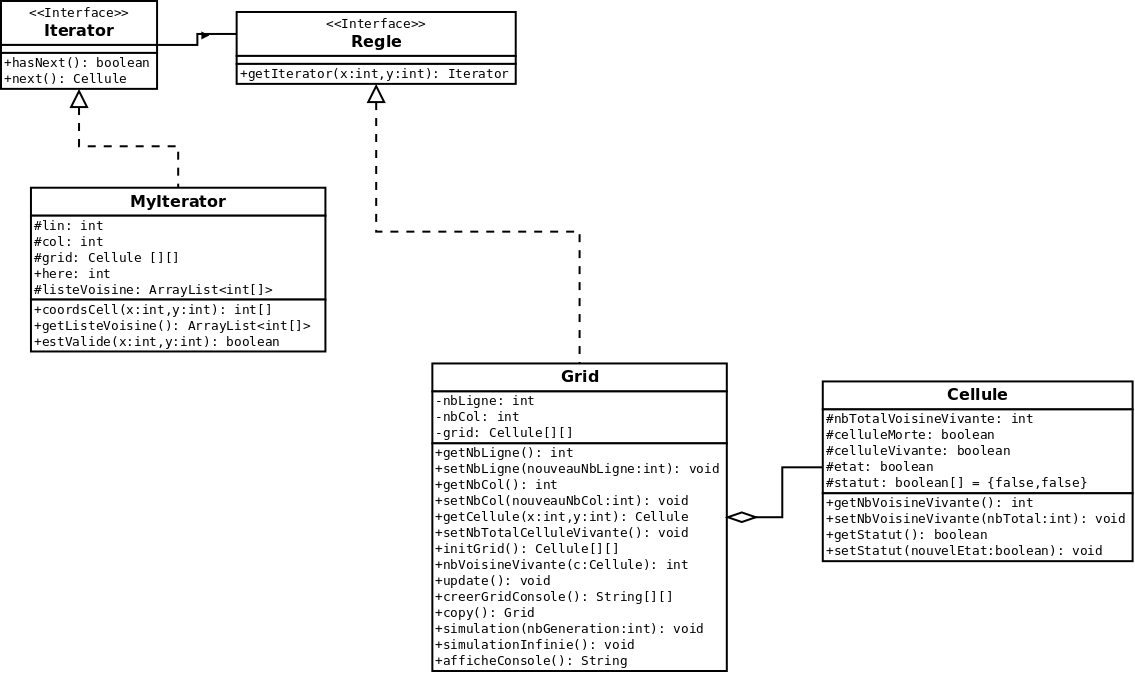
\includegraphics[scale=0.3]{images/classes.png}\\
\title{Diagramme de classe du moteur du jeu }	
\end{center}


 

\subsection{les packages}
\textbf{faire un diagramme des classes}
\section{Éléments techniques}
Comme on l'avait dit plus haut la simulation du jeu de la vie utilise une grille composer de cellules ,dans cette partie nous allons vous expliquer les points techniques du projet. Avant de coder la classe Grille nous avons définit un type cellule qui aura les arguments et les méthodes qui nous permettrons d'initialiser et de faire évoluer notre Grille future.\\

Notre moteur de jeu est basé sur une grille à deux dimensions qui représente la surface sur laquelle les cellules évolueront en fonction du nombre de leurs cellules voisines vivantes ,et pour connaitre les cellules voisines nous avons utilisé le pattern iterator de java qui nous donne le moyen de les trouver  
\subsection{Classe Cellule}

la classe cellule est un élément essentiel dans notre moteur du jeu. C'est le principal constituant de la grille et nous avons représenté une cellule par son nombre de voisines totales ,son état (true :cellule vivante, false: cellule morte ).


\subsection{Grille}
La classe Gille est celle qui utilise toutes ces classes préalablement définies, elle contient également des méthodes comme celles qui permettent de construire le grille du jeu.

La grille est la classe principale du projet,son importance réside dans le fait qu'elle permet de représenter de manière discrète l'espace dans lequel les cellules évoluent. La grille est un ensemble de cellules qui sont disposées en lignes et en colonnes, et chaque cellule peut être vivante ou morte.

Les règles du jeu de la vie sont appliquées à chaque cellule de la grille, en fonction de l'état de ses voisines immédiates. 

\subsection{L’interface graphique}
			
Pour réaliser l’interface graphique, nous avons utilisé un JFrame pour avoir une fenêtre dans laquelle on a placé au sud un JPanel qui contient  les boutons (JButton) permettant d'iteragir avec la grille. En suite au nord nous avions placé un JComponent (GridGraphique) contenant la grille.\\

GridGraphique est une classe qui hérite de JComponent à partir de laquelle nous importons les images du package Images représentant certains objets du jeu comme les cellules vivantes et les cellules mortes à la méthode chargementImages(). Chaque image est dessinée en fonction de la cellule correspondante.

\begin{center}
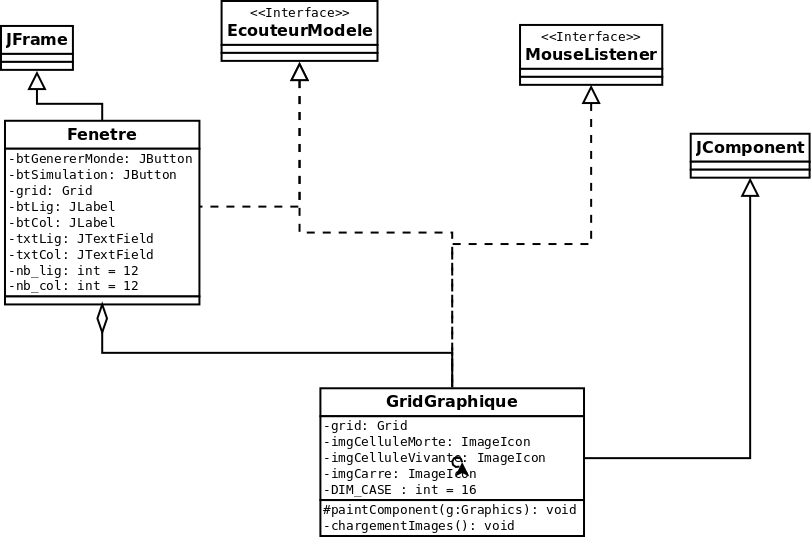
\includegraphics[scale=0.4]{images/classeIhm.png}\\
\title{Diagramme de classe Graphique}	
\end{center}	

\subsection{Manuel d'utilisation }  
Le jeu de la vie  a pour objectif principal de faire évoluer les cellules d'une génération à une autre.
\subsubsection{Jeu graphique}
Pour lancer le jeu en version graphique rendez-vous dans la racine du projet, ouvrez  un terminale et taper les commandes suivantes :
\begin{itemize}
\item ant compile 
\item ant run 
\end{itemize}

Une fois le jeu lancé vous tomberez sur la fenêtre principale(voir figure 1)
%--Afficher image Fenetre principale du jeu
\begin{center}
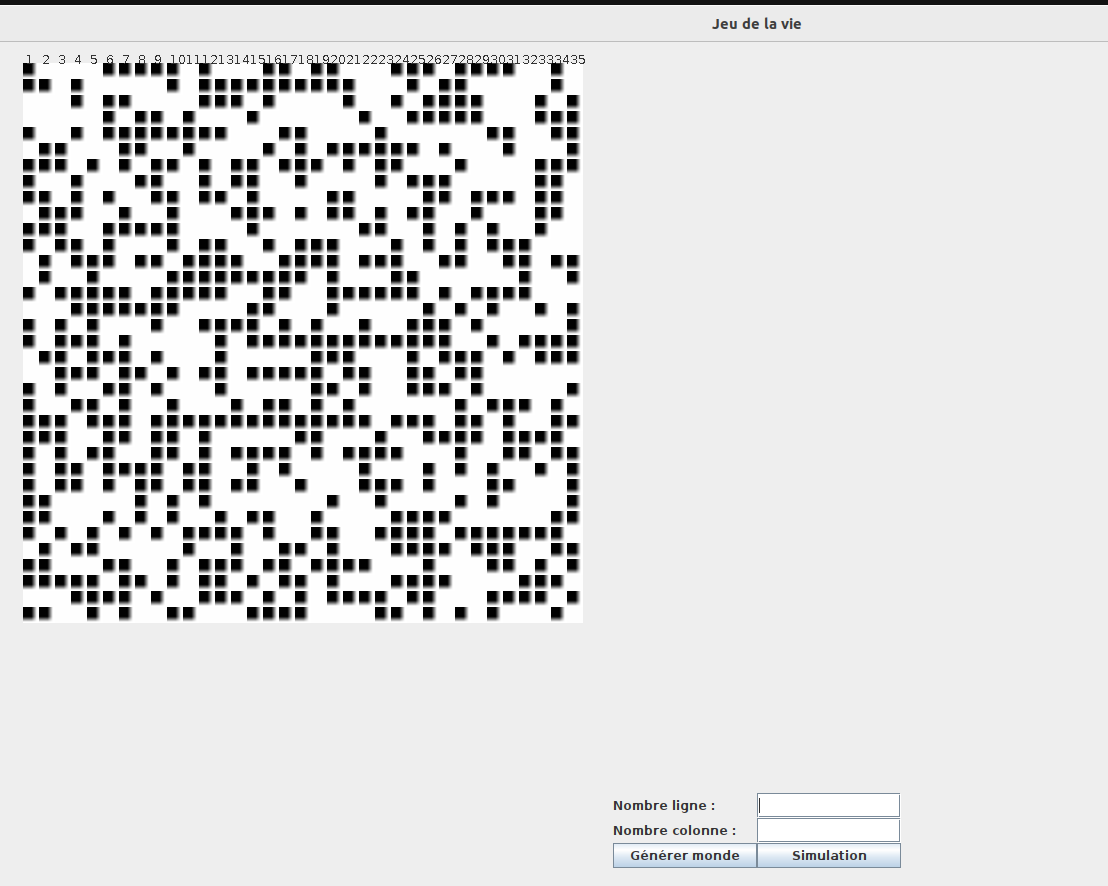
\includegraphics[scale=0.4]{./images/AffichageFenetre.png}
\title{- Figure 1 :Fenêtre principale du jeu}
\end{center}
Sur la page principale, vous pouvez faire une simulation du jeu. Vous avez deux boutons (voir figure 2):
\begin{itemize}
\item \textbf{Générer monde :}
permet de générer un monde aléatoire .
\item \textbf{Simulation :}
Permet de faire la simulation de la grille .
\end{itemize}
\begin{center}
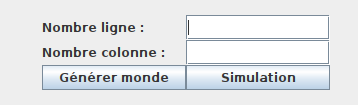
\includegraphics[scale=0.6]{./images/bouttons.png}\\
\title{Figure 2 :Les touches d'intéraction}
\end{center}

durant la simulation graphique, en arrière plan vous pouvez observez une simulation dans le terminale (voir figure : 3).
			
%--Afficher  de la grille dans la console
\begin{center}
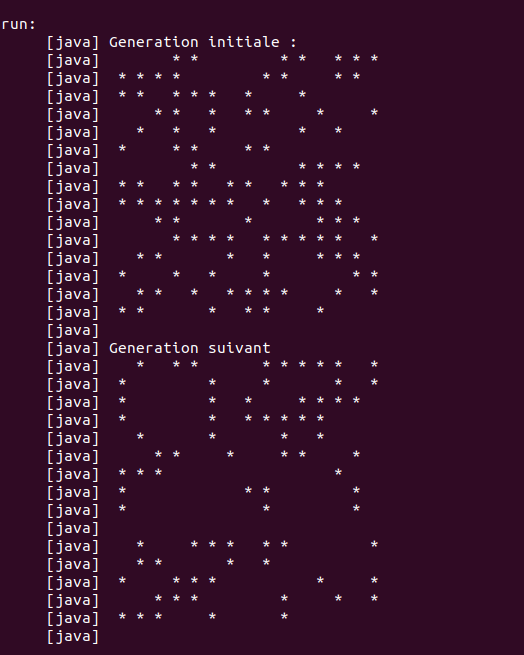
\includegraphics[scale=0.5]{./images/AffichageConsole.png}\\
\title{Figure 3 :Affichage de la grille en console}
\end{center}


			
     
%--Afficher les touches de controles

			
\subsection{Difficulté rencontrée : Algorithme HashLife}
            L'algorithme hashlife introduit la notion de macro-cellule. Une macro-cellule est une portion
        de la grille de taille $2^n.2^n$
        \\Cette portion de la grille peut être représentée par une structure de donnée quadtree. Cet algorithme permet d'accélérer la resolution une fois implémenté dans le jeu de la vie. Après plusieurs recherches sur cet algorithme notamment sur :
        \href{https://www.drdobbs.com/jvm/an-algorithm-for-compressing-space-and-t/184406478}{site de drdobbs},
        \href{https://www.dev-mind.blog/hashlife/}{Un bloc expliquant hashlife},
        Nous avons essayé de l'implémenter dans notre jeu de la vie  mais en vain.
        Dans le package hashlife se trouve la classe Noeud permettant de représenter les macro-cellules de la grille.
        




\section{conclusion} 

		La réalisation de ce projet a été une occasion pour nous membres de ce groupe d’apprendre encore plus le langage de programmation Java.
		Pendant ce projet, nous avons pu appliquer ce que nous avions appris dans les CM, les TP de ce semestre et ceux du semestre passé à savoir : la programmation orientée objet, la conception d'applications et d'autre savoir-faire. \\
D'un point de vue humain, nous avons appris à mieux travailler en équipe, à communiquer, à bien organiser un travail d'équipe et le plus important à combler nos lacunes.  
		Nous avons également appris à travailler à distance en utilisant les outils de travail de groupe comme SVN.
		
			Dans ce projet, nous avions pour objectif premier de réaliser le jeu de la vie  en implémentant toutes les règles du jeu dans une application JAVA. Nous avons donc pu coder le moteur du jeu respectant les règles du jeu, nous avons aussi réussi par faire une interface graphique afin que le jeu soit jouable graphiquement. 
			
			\subsection{Améliorations possibles   }
			
			Nous pouvons ameliorer cette application à plusieurs niveaux; tout d'abord, implémenter l'algorithme hashlife pour accélérer la resolution puis étendre ce système aux automates cellulaires neuraux.
			\\ ensuite, donner la possibilité de sauvegarder une grille de génération.
			\\L’interface graphique peut être améliorer en affichant par section pour une très grande grille de génération.
			

\end{document}